\documentclass[12pt]{article}
\usepackage{setspace, graphicx, fullpage, amssymb, amsmath, epsfig, natbib, array, multirow, hyperref}
\usepackage{amsfonts, bm} 
\usepackage{dcolumn}
\usepackage{subfigure, float} 
\usepackage[margin=1in]{geometry} 
\usepackage{verbatim}
\usepackage{url}
\usepackage{enumerate}
\usepackage{morefloats}
\newcolumntype{d}[1]{D{.}{.}{#1}} 



\begin{document}

\doublespacing
	
\section{Paper, Draft 4}

\subsection{Introduction}

Minozzi \& Volden (2013) developed the responsive extremists hypothesis which holds that party unity is typically a result of the party calling on members which leads the more extreme members to respond. While pressuring of moderates occurs, it was held that such efforts were not as common or effective as the issuance of a party call. This hypothesis relied on an assumption that both extreme and moderate members would at times have reason to vote against the majority of their party, but the extremists would be observed to be in step with the party and moderates out of step on these votes. They tested this by sorting roll call votes into party influenced votes and party free votes and estimating the impact of member ideology on decision to respond to party influence.

This paper is written with the intention of replicating this paper and extending the units of analysis to include the Senate and the period of analysis to Congresses 93-112. These extensions allow us to test the responsive extremists hypothesis in both chambers, with consideration of more recent Congresses which both chambers are held to have become more extreme. Additionally, the inclusion of the Senate allows for tests to be conducted based on proximity to reelection.

Our assumption that reelection will influence member behavior is based on a number of theories and findings on Congress. Canes-Wrone, Brady \& Cogan (2002) shows that members who stray to far from the preferences of their district are less likely to be reelected. Carson, Koger, Lebo \& Young (2010) find that voters punish members who seem to be partisan hacks.  Mayhew (1974) holds reelection to be chief among the goals of members. Levitt (1996) finds that proximity to reelection induces Senators to more strongly take their constituents' preferences into account. However, Lee (2009) holds that parties confer advantages on members through their resources and the strength of their brand.

We hypothesize that members approaching reelection will take strategic votes against the party to appear more principled to their voters. We expect this to be present primarily in votes when the party is calling, since it provides the strongest signal to constituents that a member is taking their desires into account. Still, given that the responsive extremists hypothesis was originally tested in the House (in which members are always up for reelection at the end of a Congress) we expect the effect to not be so strong as to overwhelm members' responsiveness to the party.

\subsection{Replication with Extension}

In this section we provide the results of the replication with extension to the Senate and into Congresses 93-112. To do this, we draw on Congressional roll call data for Congresses 93-112 in both chambers which we sort by party influence. Sorting is conducted by an algorithm based on the one used by Minozzi \& Volden in their original paper. This algorithm calculates the percent of times members vote in line with the majority of the party on each vote type and ideology scores based on the non-party call votes. Ideological extremism has its sign reversed for Democrats so that it takes higher values for members of both parties as they become further from the center.\footnote{A more thorough overview of the methodology is detailed in an appendix.}

We find that in both chambers and both parties, baseline party unity is most present near the party median, with a drop-off as one approaches either tail. However, party call votes demonstrate only a decline as one approaches the less extreme end of the party. This is shown in figures with $y$ axes denoting the percentage of votes cast in line with a majority of the party and $x$ axes member ideological extremism. This provides a warrant for the underlying assumptions of the responsive extremists hypothesis.

\begin{figure}[H]
	\centering
	\caption{House Rate of Voting With Party by Vote Type}
	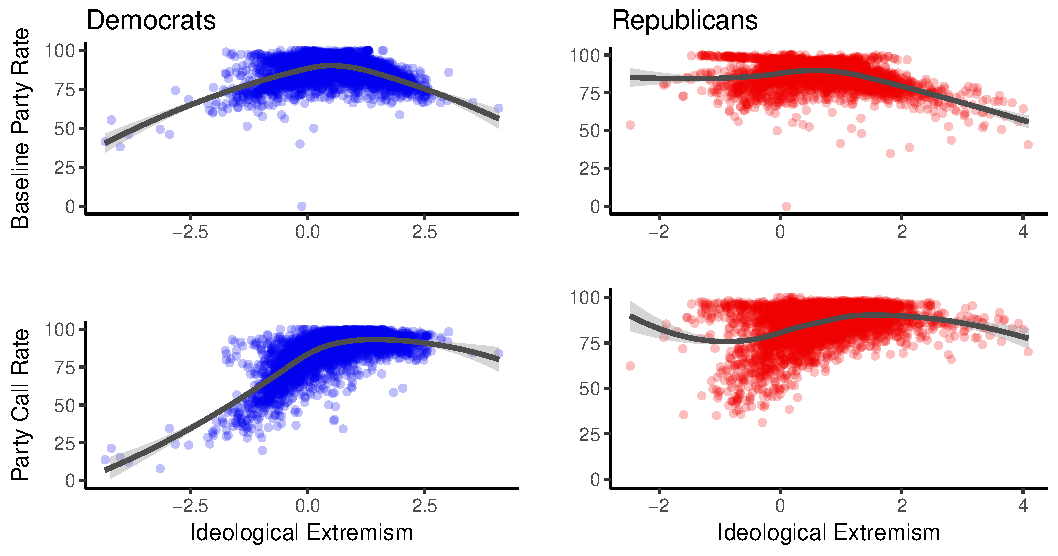
\includegraphics[width = \textwidth]{C:/Users/Ethan/Documents/GitHub/partycalls/plots/house_responsiveness_plot.pdf}
\end{figure}

\begin{figure}[H]
	\centering
	\caption{Senate Rate of Voting With Party by Vote Type}
	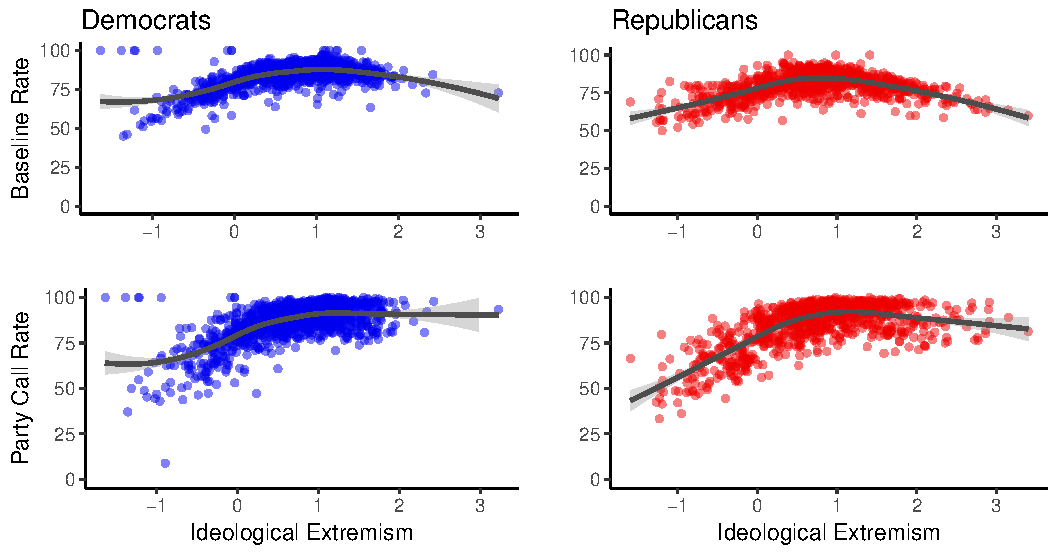
\includegraphics[width = \textwidth]{C:/Users/Ethan/Documents/GitHub/partycalls/plots/senate_responsiveness_plot.pdf}
\end{figure}

We also note that the number of party call votes in both chambers of Congress during the period of analysis are on an upward trend. We believe this trend merits further investigation, but initially take it to echo arguments such as those of Lee (2009), Theriault (2013), and Smith (2014) that Congressional parties have become more polarized over the last few decades.

\begin{figure}[H]
	\centering
	\caption{Party Calls as a Percentage of Votes, Congresses 93-112}
	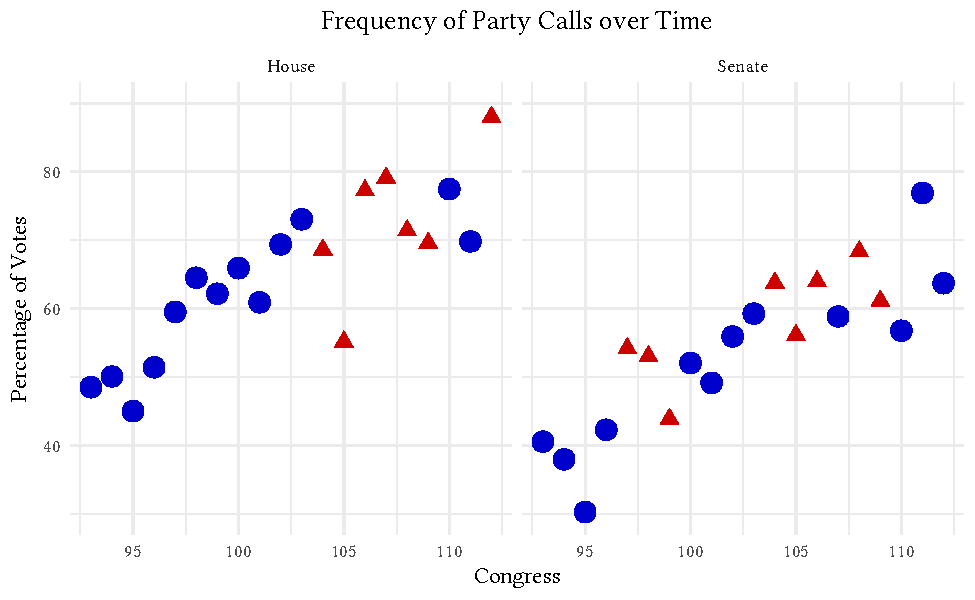
\includegraphics[width = \textwidth]{C:/Users/Ethan/Documents/GitHub/partycalls/plots/party_call_percent_both.pdf}
\end{figure}

Regression analysis with members separated by party and majority status broadly show the responsive extremists hypothesis to hold in the cases we consider. In both parties and chambers we find that increased ideological extremism leads to increased responsiveness on party call votes. In both chambers we find that southern Democrats are less responsive to the party than are other Democrats. We also note that the power committee variable we constructed for the Senate (based on membership in a top 4 committee) carries little predictive power, either in terms of substantive power or statistical significance. This is not entirely unexpected, since this is a variable we included less because we believed it had meaning to Senators and more for model comparability. We also note that in both chambers increased same party presidential vote share within one's constituency makes Democrats more likely to respond to a party call but reduces the chances of a Republican doing so.

\begin{table}[H]
	\begin{center}
		\singlespacing
		\caption{House Responsiveness to Party Calls}
		%\footnotesize
		\begin{tabular}{l c c c c }
			\hline
			& Democrats & Republicans & Majority & Minority \\
			\hline
			ideological\_extremism & $8.34^{***}$  & $5.84^{***}$  & $6.65^{***}$  & $8.73^{***}$  \\
			& $(0.17)$      & $(0.21)$      & $(0.16)$      & $(0.20)$      \\
			pfrate100              & $0.64^{***}$  & $0.41^{***}$  & $0.52^{***}$  & $0.64^{***}$  \\
			& $(0.02)$      & $(0.02)$      & $(0.01)$      & $(0.02)$      \\
			votepct                & $-0.04^{***}$ & $-0.00$       & $-0.09^{***}$ & $-0.07^{***}$ \\
			& $(0.01)$      & $(0.01)$      & $(0.01)$      & $(0.01)$      \\
			pres\_votepct          & $0.09^{***}$  & $-0.09^{***}$ & $0.20^{***}$  & $0.16^{***}$  \\
			& $(0.01)$      & $(0.02)$      & $(0.01)$      & $(0.02)$      \\
			south                  & $-2.43^{***}$ & $3.63^{***}$  & $-1.64^{***}$ & $-0.38$       \\
			& $(0.28)$      & $(0.34)$      & $(0.25)$      & $(0.31)$      \\
			female                 & $0.53$        & $-0.08$       & $-0.14$       & $2.12^{***}$  \\
			& $(0.35)$      & $(0.57)$      & $(0.40)$      & $(0.44)$      \\
			afam                   & $-0.52$       & $5.01$        & $-3.04^{***}$ & $3.25^{***}$  \\
			& $(0.44)$      & $(2.97)$      & $(0.53)$      & $(0.61)$      \\
			latino                 & $1.73^{***}$  & $2.41^{*}$    & $2.82^{***}$  & $3.02^{***}$  \\
			& $(0.51)$      & $(1.15)$      & $(0.63)$      & $(0.70)$      \\
			seniority              & $0.05$        & $-0.33^{***}$ & $0.01$        & $0.01$        \\
			& $(0.03)$      & $(0.05)$      & $(0.03)$      & $(0.04)$      \\
			freshman               & $-0.07$       & $1.00^{*}$    & $0.24$        & $-0.41$       \\
			& $(0.36)$      & $(0.46)$      & $(0.35)$      & $(0.45)$      \\
			bestgrosswart          & $-0.04^{*}$   & $-0.24^{***}$ & $-0.18^{***}$ & $-0.16^{***}$ \\
			& $(0.02)$      & $(0.03)$      & $(0.02)$      & $(0.02)$      \\
			leader                 & $1.96^{**}$   & $2.80^{***}$  & $2.61^{***}$  & $1.78^{**}$   \\
			& $(0.60)$      & $(0.76)$      & $(0.65)$      & $(0.65)$      \\
			power                  & $1.82^{***}$  & $2.95^{***}$  & $3.02^{***}$  & $1.06^{**}$   \\
			& $(0.28)$      & $(0.37)$      & $(0.27)$      & $(0.36)$      \\
			chair                  & $2.49^{***}$  & $9.85^{***}$  & $1.86^{***}$  &               \\
			& $(0.50)$      & $(0.80)$      & $(0.44)$      &               \\
			(Intercept)            & $24.00^{***}$ & $53.04^{***}$ & $36.45^{***}$ & $17.69^{***}$ \\
			& $(1.58)$      & $(2.21)$      & $(1.49)$      & $(2.05)$      \\
			\hline
			R$^2$                  & 0.63          & 0.30          & 0.57          & 0.48          \\
			Adj. R$^2$             & 0.63          & 0.30          & 0.57          & 0.48          \\
			Num. obs.              & 4746          & 3798          & 4898          & 3646          \\
			RMSE                   & 7.36          & 8.87          & 7.54          & 8.02          \\
			\hline
			\multicolumn{5}{l}{\scriptsize{$^{***}p<0.001$, $^{**}p<0.01$, $^*p<0.05$}}
		\end{tabular}
	\end{center}
\end{table}

\begin{table}[H]
	\begin{center}
		\singlespacing
		\caption{Senate Responsiveness to Party Calls}
		%\footnotesize
		\begin{tabular}{l c c c c }
			\hline
			& Democrats & Republicans & Majority & Minority \\
			\hline
			ideological\_extremism & $3.14^{***}$ & $7.79^{***}$  & $4.82^{***}$  & $7.98^{***}$ \\
			& $(0.41)$     & $(0.36)$      & $(0.31)$      & $(0.39)$     \\
			pfrate100              & $0.76^{***}$ & $0.74^{***}$  & $0.70^{***}$  & $0.72^{***}$ \\
			& $(0.03)$     & $(0.03)$      & $(0.03)$      & $(0.03)$     \\
			up\_for\_reelection    & $-0.63$      & $-1.44^{**}$  & $-0.94^{*}$   & $-0.97$      \\
			& $(0.43)$     & $(0.54)$      & $(0.41)$      & $(0.58)$     \\
			vote\_share            & $-0.05^{*}$  & $0.15^{***}$  & $-0.01$       & $0.07^{*}$   \\
			& $(0.02)$     & $(0.03)$      & $(0.02)$      & $(0.03)$     \\
			pres\_vote\_share      & $0.23^{***}$ & $-0.13^{***}$ & $0.18^{***}$  & $0.02$       \\
			& $(0.02)$     & $(0.03)$      & $(0.02)$      & $(0.03)$     \\
			south                  & $-1.69^{**}$ & $0.87$        & $-0.09$       & $1.18^{*}$   \\
			& $(0.56)$     & $(0.58)$      & $(0.42)$      & $(0.59)$     \\
			female                 & $1.69^{*}$   & $0.45$        & $0.73$        & $3.51^{**}$  \\
			& $(0.73)$     & $(1.13)$      & $(0.72)$      & $(1.07)$     \\
			afam                   & $-1.16$      & $-10.79^{*}$  & $1.32$        & $-5.19$      \\
			& $(2.79)$     & $(4.28)$      & $(4.21)$      & $(3.18)$     \\
			latino                 & $1.81$       & $7.26^{**}$   & $4.73^{*}$    & $6.06$       \\
			& $(2.20)$     & $(2.78)$      & $(1.89)$      & $(3.47)$     \\
			seniority              & $0.04$       & $-0.02$       & $0.05$        & $0.12$       \\
			& $(0.05)$     & $(0.07)$      & $(0.06)$      & $(0.07)$     \\
			freshman               & $0.77$       & $0.36$        & $0.48$        & $0.91$       \\
			& $(0.71)$     & $(0.84)$      & $(0.62)$      & $(1.00)$     \\
			retiree                & $1.60$       & $2.29^{*}$    & $1.73^{*}$    & $2.40^{*}$   \\
			& $(0.90)$     & $(1.00)$      & $(0.85)$      & $(1.07)$     \\
			best\_committee        & $0.24$       & $0.01$        & $0.03$        & $0.37^{*}$   \\
			& $(0.12)$     & $(0.15)$      & $(0.12)$      & $(0.17)$     \\
			leader                 & $2.22^{**}$  & $0.91$        & $1.51^{*}$    & $1.84^{*}$   \\
			& $(0.71)$     & $(0.78)$      & $(0.64)$      & $(0.87)$     \\
			power\_committee       & $-0.85$      & $-0.32$       & $-0.07$       & $-1.45$      \\
			& $(0.77)$     & $(0.92)$      & $(0.71)$      & $(1.02)$     \\
			chair                  & $0.85$       & $3.63^{***}$  & $0.21$        & $-10.87$     \\
			& $(0.54)$     & $(0.70)$      & $(0.51)$      & $(7.70)$     \\
			(Intercept)            & $9.45^{**}$  & $18.18^{***}$ & $16.69^{***}$ & $8.74^{*}$   \\
			& $(2.91)$     & $(3.49)$      & $(2.63)$      & $(3.83)$     \\
			\hline
			R$^2$                  & 0.69         & 0.64          & 0.68          & 0.62         \\
			Adj. R$^2$             & 0.68         & 0.64          & 0.67          & 0.61         \\
			Num. obs.              & 1042         & 951           & 1100          & 893          \\
			RMSE                   & 6.12         & 7.25          & 5.91          & 7.67         \\
			\hline
			\multicolumn{5}{l}{\scriptsize{$^{***}p<0.001$, $^{**}p<0.01$, $^*p<0.05$}}
		\end{tabular}
	\end{center}
\end{table}

In Table 2, we see some evidence of differences between members up for reelection and others. Though it fails to meet traditional significance threshold for Democrats, across all subgroups this coefficient is negative. 

\subsection{Reelection in the Senate}

In this section we test specifically for differences in member responsiveness by proximity to reelection. In order to do this, we estimate models which rely on same-state Senator pairs when one of them is up for reelection at the end of the Congress. These pairings are ideal since an expectation is that members will respond according to their voters and same-state Senators are elected by the same voters. So, we assume that these pairs will change their behavior in comparable ways as reelection approaches. 

The fact that same-state Senators are not up for reelection at the same time allows us to estimate a generalization of a difference-in-differences design on pairs in Congresses which one is up for reelection. We use this to compare member responsiveness to the party on party calls, the baseline rate of voting with the party, and the difference between these two quantities between the member up for reelection and the member in the beginning or middle of their term. For each of these a placebo test with randomly assigned treatment is also shown.\footnote{Reported 95\% confidence intervals are the result of bootstrapping by states. Further details about the tests can be found in an appendix.} Cases which have more than two Senators from a state (due to deaths and retirements) are dropped from the analysis.

\begin{figure}[H]
	\centering
	\caption{Senate Rate of Voting With Party by Vote Type}
	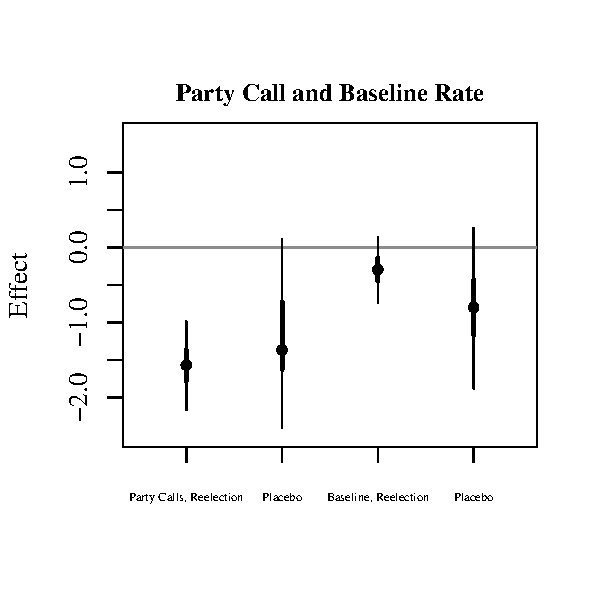
\includegraphics[width = 10cm]{C:/Users/Ethan/Documents/GitHub/partycalls/plots/senate-diff-in-diff-coeff-separate.pdf}
\end{figure}

\begin{figure}[H]
	\centering
	\caption{Senate Rate of Voting With Party by Vote Type}
	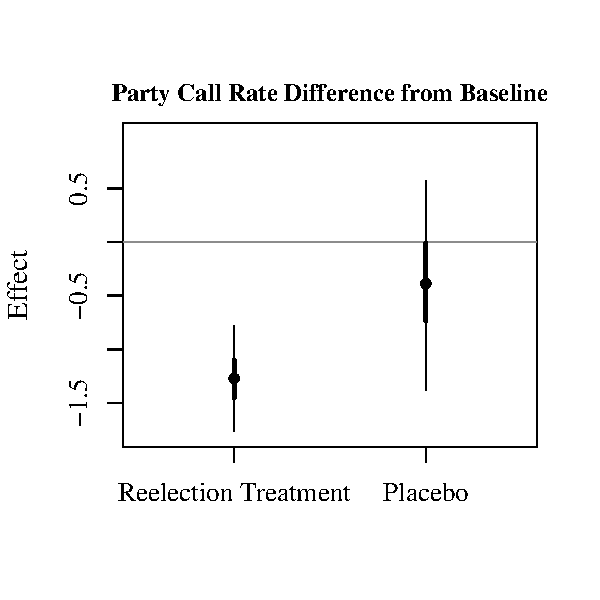
\includegraphics[width = 10cm]{C:/Users/Ethan/Documents/GitHub/partycalls/plots/senate-diff-in-diff-coeff.pdf}
\end{figure}

The results of these tests clearly show that member responsiveness to party calls declines, on average, about 1.5\% when they are up for reelection at the end of a Congress. Since the average number of party calls in a Congress during the time we analyze is approximately 365, this means that a Senate party can generally expect to count on members up for reelection for a little over 5 votes against the party's position on party call votes. This would be enough to allow them to point to multiple instances in which they went against the party to their voters without greatly hindering the party's goals. Member voting behavior on other votes does not exhibit this relationship, likely due to them not being perceived as providing as clear of a signal to voters. Thus, we conclude that member proximity to reelection leads members to place greater weight on voter desires while balancing them against those of the party.

\subsection{Conclusion}

In this paper, we tested if members respond to party calls in the Senate as they do in the House, using similar analyses to Minozzi \& Volden (2013). We found that while there was variation between members based on majority status, chamber, and party, that the responsive extremists hypothesis held in this extended set of cases. Further, in the Senate we are able to consider the role that proximity to reelection has in responsiveness to the party in Congress. Across differing tests we find that in Congresses which a member is up for reelection they are less likely to vote with a majority of the party on party call votes, but not on other vote types. This is in line with expectations of members working to consider voter preferences more highly as reelection becomes more proximate, though it expands on previous studies by highlighting specific conditions under which member behavior changes and others which it remains constant.

\pagebreak

\section{Appendices}

\subsection{Appendix A: Detailing the New Sorting Algorithm}

As in Minozzi \& Volden (2013) we develop an algorithm to sort votes based on the degree to which vote choice can be significantly predicted by party when vote choice is modeled by party and ideology. This algorithm works iteratively, with member ideology in one iteration calculated on the votes which were not party calls in the previous iteration, with the ideology for the first iteration being set as votes which have more than 65\% or less than 35\% of members voting on a bill on the same side. The algorithm must run 15 iterations per Congress as a burn-in period. Once this period has concluded the algorithm continues either until the number of votes switched has hit a minimum and begun to climb or until there are fewer than 5 votes which switch between iterations. Once these conditions are met, it continues for 15 additional iterations, the last 5 of which are used to identify party calls and non calls. Any votes which switched between party calls and non party calls during the final five iterations are dropped from our analyses.

We find that the results produced by the algorithm largely do not involve a tradeoff of party and ideology explaining votes, but instead typically have both explaining effects in the same direction. We have made some changes to this algorithm, which are detailed below.

% latex table generated in R 3.3.2 by xtable 1.8-2 package
% Thu Feb 23 17:39:42 2017
\begin{table}[H]
	\centering
	\caption{House Sorting Algorithm Coefficient Signs}
	\begin{tabular}{rrr}
		\hline
		& ($-$) Ideal & (+) Ideal \\ 
		\hline
		(-) Party & 0.38 & 0.15 \\ 
		(+) Party & 0.17 & 0.30 \\ 
		\hline
	\end{tabular}
\end{table}

% latex table generated in R 3.3.2 by xtable 1.8-2 package
% Thu Feb 23 17:23:31 2017
\begin{table}[H]
	\centering
	\caption{Senate Sorting Algorithm Coefficient Signs}
	\begin{tabular}{rrr}
		\hline
		& ($-$) Ideal & (+) Ideal \\ 
		\hline
		($-$) Party & 0.33 & 0.16 \\ 
		(+) Party & 0.23 & 0.28 \\ 
		\hline
	\end{tabular}
\end{table}

One of the key changes was the use of the \verb|emIRT()| R function as described in Imai, Lo \& Olmsted (2016) in order to obtain members' party free ideology. This function was developed by Imai and co-authors in order to produce estimates analagous to those of the \verb|ideal()| function developed by Clinton, Jackman \& Rivers (2004), which was used by Minozzi \& Volden (2013). A key advantage of this new function for estimation of member ideology is that it produces results with greatly reduced computation.

We found that the lowered number of both members and bills in the Senate required a few changes to the vote sorting method. First, since p-values will necessarily be lower with fewer observations, we had to change the p-value threshold for party significance to 0.05 (from 0.01). Next, since the ideal point algorithm uses a logistic regression problems arose in vote sorting when we also tried to use a logistic regression in the Senate and changed to using a linear model. Neither change leads the sorting in the House to change drastically and we find that the sorting of votes based on whether they are close or lopsided mirrors that found in Minozzi \& Volden (2013) very closely.

% latex table generated in R 3.3.2 by xtable 1.8-2 package
% Mon Mar 20 13:02:44 2017
\begin{table}[H]
	\centering
	\caption{House Vote Coding for Close and Lopsided Votes} 
	\begin{tabular}{lrr}
		\hline
		& Party Call & Noncall \\ 
		\hline
		Lopsided & 4245 & 6123 \\ 
		Close & 9308 & 1090 \\ 
		\hline
	\end{tabular}
\end{table}

% latex table generated in R 3.3.2 by xtable 1.8-2 package
% Mon Mar 20 13:04:18 2017
\begin{table}[H]
	\centering
	\caption{Senate Vote Coding for Close and Lopsided Votes} 
	\begin{tabular}{lrr}
		\hline
		& Party Call & Noncall \\ 
		\hline
		Lopsided & 2063 & 4876 \\ 
		Close & 5233 & 1851 \\ 
		\hline
	\end{tabular}
\end{table}













\subsection{Appendix B: Methodology for Senate Reelection Section}

In order to better test the role of reelection we use same-state senators as a natural pairing. We view this as an ideal pairing since they answer to the same possible set of voters and therefore should have similar preferences induced by proximity to reelection. The tests we performed on these pairs were generalizations of the difference in differences design in which the member not up for reelection had their response rate subtracted from that of the member who was up for reelection for the first figure in the paper and for the second members had the difference between their party call response rate and baseline rate of voting with the party subtracted from that of the other Senator from their state under the same conditions. 

Here we show the effects in tables, along with breakdowns by seat pair type. We additionally show the results of a model with fixed effects by member and Congress. This produces substantively similar effects to those reported in the main paper on the effects of being up for reelection and changes in ideological extremism. This is presented as a robustness check for the results we present in the paper.

% latex table generated in R 3.3.2 by xtable 1.8-2 package
% Mon Mar 27 22:28:47 2017
\begin{table}[H]
	\centering
	\caption{Reelection and Response to Party Calls, Difference in Differences} 
	\begin{tabular}{llrrr}
		\hline
		test & DV & Estimate & Lower\_Bound & Upper\_Bound \\ 
		\hline
		Effect & pirate100 & -1.569 & -2.139 & -1.001 \\ 
		Placebo & pirate100 & -0.331 & -1.281 & 1.259 \\ 
		Effect & pfrate100 & -0.297 & -0.798 & 0.126 \\ 
		Placebo & pfrate100 & -0.644 & -1.074 & 1.143 \\ 
		\hline
	\end{tabular}
\end{table}

% latex table generated in R 3.3.2 by xtable 1.8-2 package
% Mon Mar 27 22:28:47 2017
\begin{table}[H]
	\centering
	\caption{Diff in Diff, Subgroup Condition, Party Influenced Rate} 
	\begin{tabular}{llr}
		\hline
		Test & DV & Estimate \\ 
		\hline
		2 Maj Dems Effect & pirate100 & 0.0708958 \\ 
		2 Maj Dems Placebo & pirate100 & 0.0859113 \\ 
		2 Min Dems Effect & pirate100 & -1.8733904 \\ 
		2 Min Dems Placebo & pirate100 & 0.1595294 \\ 
		2 Maj Reps Effect & pirate100 & -1.1307379 \\ 
		2 Maj Reps Placebo & pirate100 & 0.1677148 \\ 
		2 Min Reps Effect & pirate100 & 0.3990873 \\ 
		2 Min Reps Placebo & pirate100 & -0.1514964 \\ 
		Split, Maj Dem, Dem Effect & pirate100 & 3.8789004 \\ 
		Split, Maj Dem, Dem Placebo & pirate100 & -40.3593458 \\ 
		Split, Maj Dem, Rep Effect & pirate100 & -8.6767819 \\ 
		Split, Maj Dem, Rep Placebo & pirate100 & -42.2647881 \\ 
		Split, Maj Rep, Dem Effect & pirate100 & -8.0169523 \\ 
		Split, Maj Rep, Dem Placebo & pirate100 & -42.4436232 \\ 
		Split, Maj Rep, Rep Effect & pirate100 & 0.0096892 \\ 
		Split, Maj Rep, Rep Placebo & pirate100 & -44.6050484 \\ 
		\hline
	\end{tabular}
\end{table}

% latex table generated in R 3.3.2 by xtable 1.8-2 package
% Sun Mar 26 19:10:24 2017
\begin{table}[H]
	\centering
	\caption{Reelection and Response to Party Calls, Difference in Differences} 
	\begin{tabular}{llrrr}
		\hline
		test & DV & Estimate & Lower\_Bound & Upper\_Bound \\ 
		\hline
		Effect & pirate100 - pfrate100 & -1.272 & -1.775 & -0.794 \\ 
		Placebo & pirate100 - pfrate100 & -0.292 & -0.904 & 0.935 \\ 
		\hline
	\end{tabular}
\end{table}

% latex table generated in R 3.3.2 by xtable 1.8-2 package
% Sun Mar 26 19:10:27 2017
\begin{table}[H]
	\centering
	\caption{Diff in Diff, Subgroup Condition, Party Influenced Rate} 
	\begin{tabular}{llr}
		\hline
		Test & DV & Estimate \\ 
		\hline
		2 Maj Dems Effect & pirate100 - pfrate100 & -0.1191943 \\ 
		2 Maj Dems Placebo & pirate100 - pfrate100 & 0.5657017 \\ 
		2 Min Dems Effect & pirate100 - pfrate100 & -1.8253378 \\ 
		2 Min Dems Placebo & pirate100 - pfrate100 & -0.4463733 \\ 
		2 Maj Reps Effect & pirate100 - pfrate100 & -2.2112471 \\ 
		2 Maj Reps Placebo & pirate100 - pfrate100 & -0.1749949 \\ 
		2 Min Reps Effect & pirate100 - pfrate100 & 0.7774782 \\ 
		2 Min Reps Placebo & pirate100 - pfrate100 & -0.4516436 \\ 
		Split, Maj Dem, Dem Effect & pirate100 - pfrate100 & -0.8756821 \\ 
		Split, Maj Dem, Dem Placebo & pirate100 - pfrate100 & -1.8454871 \\ 
		Split, Maj Dem, Rep Effect & pirate100 - pfrate100 & -1.4582552 \\ 
		Split, Maj Dem, Rep Placebo & pirate100 - pfrate100 & 0.0117995 \\ 
		Split, Maj Rep, Dem Effect & pirate100 - pfrate100 & -7.1166813 \\ 
		Split, Maj Rep, Dem Placebo & pirate100 - pfrate100 & -3.4630959 \\ 
		Split, Maj Rep, Rep Effect & pirate100 - pfrate100 & 0.3772151 \\ 
		Split, Maj Rep, Rep Placebo & pirate100 - pfrate100 & 0.2964502 \\ 
		\hline
	\end{tabular}
\end{table}

\begin{table}[H]
	\begin{center}
		\caption{Senate Fixed Effects Models, Party Call Response Rate}
		\begin{tabular}{l c c c c }
			\hline
			& Democrats & Republicans & Majority & Minority \\
			\hline
			Ideological Extremism  & $2.88^{***}$ & $4.00^{***}$  & $1.80^{**}$   & $3.93^{***}$ \\
			& $(0.69)$     & $(0.75)$      & $(0.64)$      & $(0.97)$     \\
			Baseline Rate of Voting with Party               & $0.37^{***}$ & $0.25^{***}$  & $0.37^{***}$  & $0.18^{*}$   \\
			& $(0.05)$     & $(0.05)$      & $(0.05)$      & $(0.07)$     \\
			Up For Reelection     & $-0.55^{*}$  & $-1.55^{***}$ & $-1.02^{***}$ & $-1.04^{**}$ \\
			& $(0.27)$     & $(0.34)$      & $(0.28)$      & $(0.37)$     \\
			Vote Share             & $0.03$       & $-0.05$       & $0.02$        & $-0.02$      \\
			& $(0.02)$     & $(0.03)$      & $(0.03)$      & $(0.04)$     \\
			Presidential Vote Share       & $0.27^{***}$ & $0.09$        & $0.31^{***}$  & $0.14^{*}$   \\
			& $(0.04)$     & $(0.05)$      & $(0.06)$      & $(0.06)$     \\
			Freshman                & $0.71$       & $0.98^{*}$    & $0.77$        & $0.78$       \\
			& $(0.48)$     & $(0.46)$      & $(0.46)$      & $(0.76)$     \\
			Retiree                 & $0.25$       & $0.88$        & $0.36$        & $0.75$       \\
			& $(0.83)$     & $(0.83)$      & $(0.99)$      & $(0.91)$     \\
			Best Committee         & $0.14$       & $0.11$        & $0.29$        & $0.36^{*}$   \\
			& $(0.12)$     & $(0.16)$      & $(0.15)$      & $(0.18)$     \\
			Power Committee        & $-0.48$      & $-0.22$       & $-1.26$       & $-0.45$      \\
			& $(0.70)$     & $(0.98)$      & $(0.89)$      & $(1.01)$     \\
			Leader                  & $0.87$       & $1.46^{*}$    & $1.39$        & $1.31$       \\
			& $(0.47)$     & $(0.62)$      & $(0.78)$      & $(0.80)$     \\
			Committee Chair                   & $0.38$       & $0.65$        & $-0.57$       &              \\
			& $(0.64)$     & $(0.71)$      & $(0.56)$      &              \\
			\hline
			Num. obs.               & 1042         & 951           & 1052          & 843          \\
			R$^2$      & 0.89         & 0.91          & 0.92          & 0.94         \\
			Adj. R$^2$ & 0.87         & 0.88          & 0.89          & 0.91         \\
			\hline
			\multicolumn{5}{l}{\scriptsize{$^{***}p<0.001$, $^{**}p<0.01$, $^*p<0.05$}}
		\end{tabular}
	\end{center}
\end{table}

\subsection{Appendix C: Other Tables and Figures from Replication}
\begin{table}
	\begin{center}
		\caption{Statistical models}
		\begin{tabular}{l c c c c c c }
			\hline
			& \multicolumn{3}{c}{Democrats} & \multicolumn{3}{c}{Republicans} \\
			\cline{2-7}
			& 97th & 102nd & 107th & 97th & 102nd & 107th \\
			\hline
			ideological\_extremism & $9.27^{***}$  & $5.07^{***}$  & $-1.11$      & $5.21^{***}$ & $6.78^{***}$  & $-0.20$       \\
			& $(0.53)$      & $(0.69)$      & $(1.50)$     & $(0.71)$     & $(0.76)$      & $(0.61)$      \\
			pfrate100              & $1.03^{***}$  & $0.67^{***}$  & $1.11^{**}$  & $0.50^{***}$ & $0.48^{***}$  & $0.35^{**}$   \\
			& $(0.07)$      & $(0.08)$      & $(0.36)$     & $(0.08)$     & $(0.08)$      & $(0.11)$      \\
			pres\_votepct          & $0.15^{**}$   & $0.14^{**}$   & $0.22^{***}$ & $0.23^{***}$ & $0.21^{*}$    & $0.18^{***}$  \\
			& $(0.05)$      & $(0.05)$      & $(0.06)$     & $(0.07)$     & $(0.08)$      & $(0.03)$      \\
			south                  & $-4.20^{***}$ & $-1.31$       & $-3.13^{*}$  & $1.53$       & $0.07$        & $1.75^{***}$  \\
			& $(1.02)$      & $(0.80)$      & $(1.28)$     & $(1.19)$     & $(1.22)$      & $(0.52)$      \\
			votepct                & $-0.08^{*}$   & $-0.03$       & $-0.04$      & $0.05$       & $-0.00$       & $-0.03$       \\
			& $(0.03)$      & $(0.03)$      & $(0.05)$     & $(0.05)$     & $(0.03)$      & $(0.02)$      \\
			female                 & $0.05$        & $-1.58$       & $2.44^{*}$   & $-4.21^{*}$  & $-1.87$       & $-1.39$       \\
			& $(2.06)$      & $(1.22)$      & $(1.21)$     & $(2.00)$     & $(2.25)$      & $(0.83)$      \\
			afam                   & $-2.56$       & $-1.98$       & $-1.43$      &              & $3.95$        & $-3.54$       \\
			& $(2.12)$      & $(1.58)$      & $(1.73)$     &              & $(6.14)$      & $(3.57)$      \\
			latino                 & $4.02$        & $2.79$        & $0.69$       & $-1.28$      & $3.26$        & $0.79$        \\
			& $(2.91)$      & $(1.90)$      & $(1.89)$     & $(5.75)$     & $(6.35)$      & $(1.50)$      \\
			seniority              & $0.08$        & $0.07$        & $-0.11$      & $-0.02$      & $-0.71^{***}$ & $-0.17^{*}$   \\
			& $(0.12)$      & $(0.10)$      & $(0.13)$     & $(0.17)$     & $(0.15)$      & $(0.08)$      \\
			freshman               & $-1.25$       & $0.01$        & $-0.13$      & $3.45^{*}$   & $3.76^{*}$    & $0.59$        \\
			& $(1.43)$      & $(1.19)$      & $(2.02)$     & $(1.34)$     & $(1.77)$      & $(0.78)$      \\
			bestgrosswart          & $0.09$        & $-0.06$       & $0.25^{*}$   & $0.11$       & $0.11$        & $0.17^{**}$   \\
			& $(0.08)$      & $(0.08)$      & $(0.10)$     & $(0.09)$     & $(0.11)$      & $(0.05)$      \\
			leader                 & $7.02^{*}$    & $2.00$        & $0.56$       & $0.38$       & $4.26$        & $3.17^{*}$    \\
			& $(2.87)$      & $(1.95)$      & $(2.42)$     & $(2.42)$     & $(2.24)$      & $(1.23)$      \\
			power                  & $1.09$        & $1.44$        & $-1.23$      & $-1.37$      & $-0.03$       & $-0.21$       \\
			& $(1.02)$      & $(0.90)$      & $(1.31)$     & $(1.35)$     & $(1.41)$      & $(0.63)$      \\
			chair                  & $2.61$        & $1.31$        &              &              &               & $1.30$        \\
			& $(1.52)$      & $(1.35)$      &              &              &               & $(0.91)$      \\
			(Intercept)            & $-18.03^{**}$ & $25.29^{***}$ & $-33.70$     & $11.17$      & $23.11^{**}$  & $47.81^{***}$ \\
			& $(6.71)$      & $(7.32)$      & $(35.43)$    & $(8.06)$     & $(8.49)$      & $(10.27)$     \\
			\hline
			R$^2$                  & 0.82          & 0.65          & 0.36         & 0.54         & 0.61          & 0.52          \\
			Adj. R$^2$             & 0.80          & 0.64          & 0.31         & 0.50         & 0.58          & 0.49          \\
			Num. obs.              & 233           & 263           & 209          & 187          & 162           & 217           \\
			RMSE                   & 5.47          & 4.97          & 6.39         & 5.62         & 5.86          & 3.26          \\
			\hline
			\multicolumn{7}{l}{\scriptsize{$^{***}p<0.001$, $^{**}p<0.01$, $^*p<0.05$}}
		\end{tabular}
	\end{center}
\end{table}

\begin{figure}[H]
	\centering
	\caption{House Ideological Extremism Coefficient Plot}
	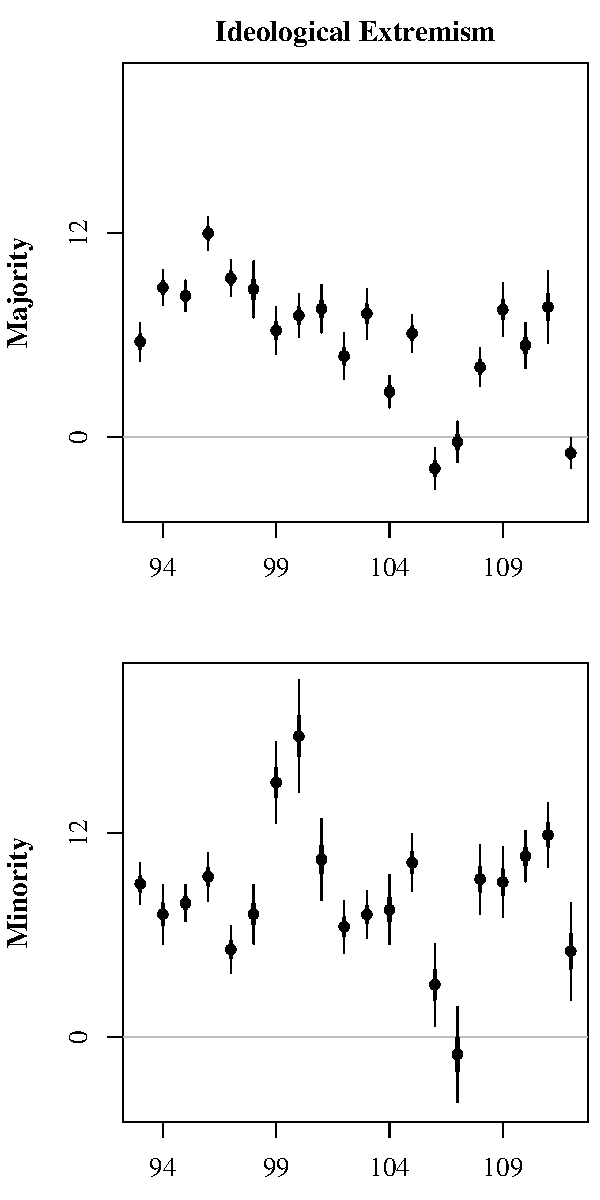
\includegraphics[width = 10cm]{C:/Users/Ethan/Documents/GitHub/partycalls/plots/who-heeds-figure2-replication_lm.pdf}
\end{figure}

\begin{figure}[H]
	\centering
	\caption{Senate Ideological Extremism Coefficient Plot}
	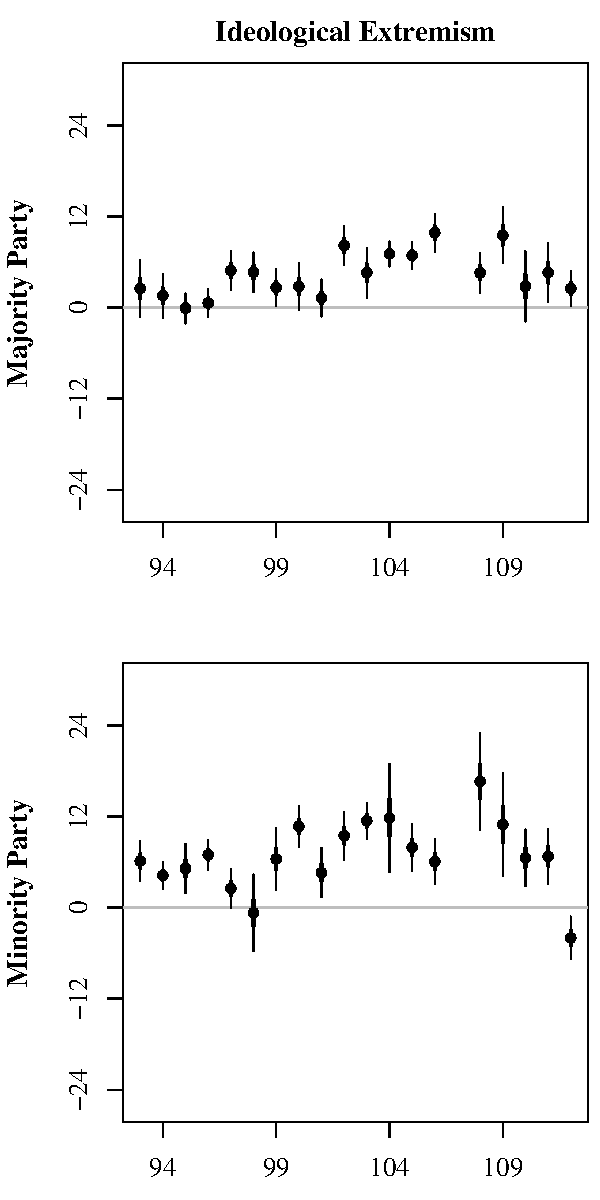
\includegraphics[width = 10cm]{C:/Users/Ethan/Documents/GitHub/partycalls/plots/senate-figure2-lm.pdf}
\end{figure}





















































\end{document}